% Bibliography report, Team 1. Build: cd docs/literature && latexmk -pdf literature_report.tex
\documentclass[11pt,a4paper]{article}
\usepackage[T1]{fontenc}
\usepackage{mathptmx}
\usepackage[margin=2.5cm]{geometry}
\usepackage{graphicx}
\usepackage{booktabs}
\usepackage{tabularx}
\usepackage{array}
\usepackage{enumitem}
\usepackage{titlesec}
\usepackage[hidelinks]{hyperref}
\usepackage{xcolor}
\usepackage{cite}
\setlength{\parindent}{0pt}
\setlength{\parskip}{6pt}
\setlist{nosep,leftmargin=*}
\titleformat{\section}{\Large\bfseries}{\thesection}{1em}{}
\titleformat{\subsection}{\large\bfseries}{\thesubsection}{1em}{}
\titleformat{\subsubsection}{\normalsize\bfseries}{\thesubsubsection}{1em}{}
\newcolumntype{L}{>{\raggedright\arraybackslash}X}
\newcommand{\source}[3]{\paragraph*{#1}\mbox{}\\\textit{#2}~#3\par}
\newcommand{\relevance}[1]{\par\textbf{Relevance to our project:} #1\par}
\graphicspath{{../img/}}

\begin{document}

% ---------------- Title page ----------------
\begin{titlepage}
\centering
{\large Technische Hochschule Deggendorf\par}
\vspace{1.2cm}
{\large MDM-M-2 Case Study Intelligent Systems in Production\par}
\vspace{2cm}
{\LARGE\bfseries Binary Classification of AOI Alarms into\\[4pt] True Defects and False Calls\par}
\vspace{0.4cm}
{\large Second check of AOI results with supervised machine learning\\(Siemens production data)\par}
\vspace{1.5cm}
{\Large\bfseries Bibliography Report\par}
\vspace{2cm}
{\large Team 1\par}
\vspace{0.3cm}
Yu Han (team lead)\\
Melisa Subasi\\
Meron Hagos\\
Alejandro Rivas\par
\vspace{1.5cm}
Under the supervision of:\\
Prof.\ Dr.-Ing.\ Hamidreza Heidari\par
\vspace{0.6cm}
Date of submission: 03.11.2026\par
\vfill
{\small Literature parts: M.~Subasi (AOI and false calls), M.~Hagos (classifiers), A.~Rivas (evaluation).\\
Report compiled and edited by Y.~Han. Code and data: \url{https://github.com/bodhi584/aoi-false-call-classification}\par}
\end{titlepage}
\pagenumbering{roman}

% ---------------- Abstract ----------------
\section*{Abstract}
\addcontentsline{toc}{section}{Abstract}
Electronics manufacturers aim at zero defects, so every assembled circuit board is checked by automated optical inspection (AOI). AOI compares camera measurements of each solder joint with fixed limits and sends every flagged board to a manual inspection station. Most of these alarms are false calls: in the public Siemens production data used in our project, 97.8\,\% of the flagged boards have no real defect. Manual re-inspection of good boards costs operator time, and Siemens is working on the same problem in its Erlangen electronics factory today.

This report reviews 14 sources, from the general to the specific: zero-defect manufacturing and AOI in electronics assembly, the false-call problem and the Siemens data set, earlier studies that use supervised machine learning as a second check of AOI results, and methods to evaluate a classifier on imbalanced classes and on production data that change over time. The literature shows that classifiers such as random forests and neural networks can recognise false calls from AOI measurements. However, most studies use small or unpublished data and standard metrics, and they do not test the models in time order. One study on the same Siemens data shows that models that meet a 1\,\% missed-defect goal on a random test set miss 5--15\,\% of the defects on later production days.

From this review we take the methods for our project (binary classification with logistic regression, random forest and a neural network; recall and specificity; a decision threshold for 99\,\% recall; evaluation day by day in time order) and the gap that our project addresses: evaluation in time order with a fixed minimum recall for true defects.

\newpage
\tableofcontents
\listoffigures
\listoftables
\newpage

% ---------------- Introduction ----------------
\pagenumbering{arabic}
\section{Introduction}
Quality control is a core task of production management. In electronics assembly, components are soldered onto printed circuit boards by surface-mount technology (SMT), and one bad solder joint can make a whole product fail. Automated optical inspection is therefore placed after soldering. AOI is fast and checks every joint, but it is tuned to miss no defect, so it raises many false alarms (false calls). Each alarm is checked again by an operator at a manual inspection station. This report reviews the literature on this problem as the basis of our case study.

\subsection{Objectives}
\begin{itemize}
  \item Describe why AOI produces false calls and why this matters for production (background).
  \item Review earlier work that uses supervised machine learning as a second check of AOI results.
  \item Review how such a classifier should be evaluated when true defects are rare and the production line changes over time.
  \item Derive the methods of our project and the research gap it addresses.
\end{itemize}

\subsection{Scope of the review}
The review covers 14 sources published between 2001 and 2026: peer-reviewed journal and conference papers, one data article, one preprint and one industry press release. It is limited to AOI of solder joints in SMT assembly and to tabular AOI measurements; image-based defect detection with deep learning is outside the scope, because our project starts after the AOI machine has already made its measurements.

% ---------------- Materials and Methods ----------------
\section{Materials and Methods}

\subsection{Method of the literature search}
The three literature topics were split among three team members; each member searched, read and summarised 3--4 sources, and the team lead checked every reference and merged the parts into this report.
\begin{itemize}
  \item \textbf{Databases:} IEEE Xplore, ScienceDirect, SpringerLink, ACM Digital Library, arXiv, Google Scholar, Mendeley Data and the Siemens press room.
  \item \textbf{Search terms:} \textit{automated optical inspection}, \textit{false call}, \textit{SMT}, \textit{solder joint}, \textit{machine learning}, \textit{random forest}, \textit{imbalanced data}, \textit{ROC analysis}, \textit{concept drift}.
  \item \textbf{Inclusion criteria:} the source deals with AOI false calls, with the Siemens AOI data, or with a method we use; it is peer-reviewed or a primary source (data article, company press release); its full reference can be verified (DOI or official page).
  \item \textbf{Reading:} for each source we noted what was done, the data, the main result and how it relates to our project. Numbers are only taken from the sources themselves or from our own result files.
\end{itemize}

\subsection{Reviewed literature}
Figure~\ref{fig:map} shows how the sources are ordered, from the general background to the specific question of our project. The following subsections follow this order.

\begin{figure}[h]
  \centering
  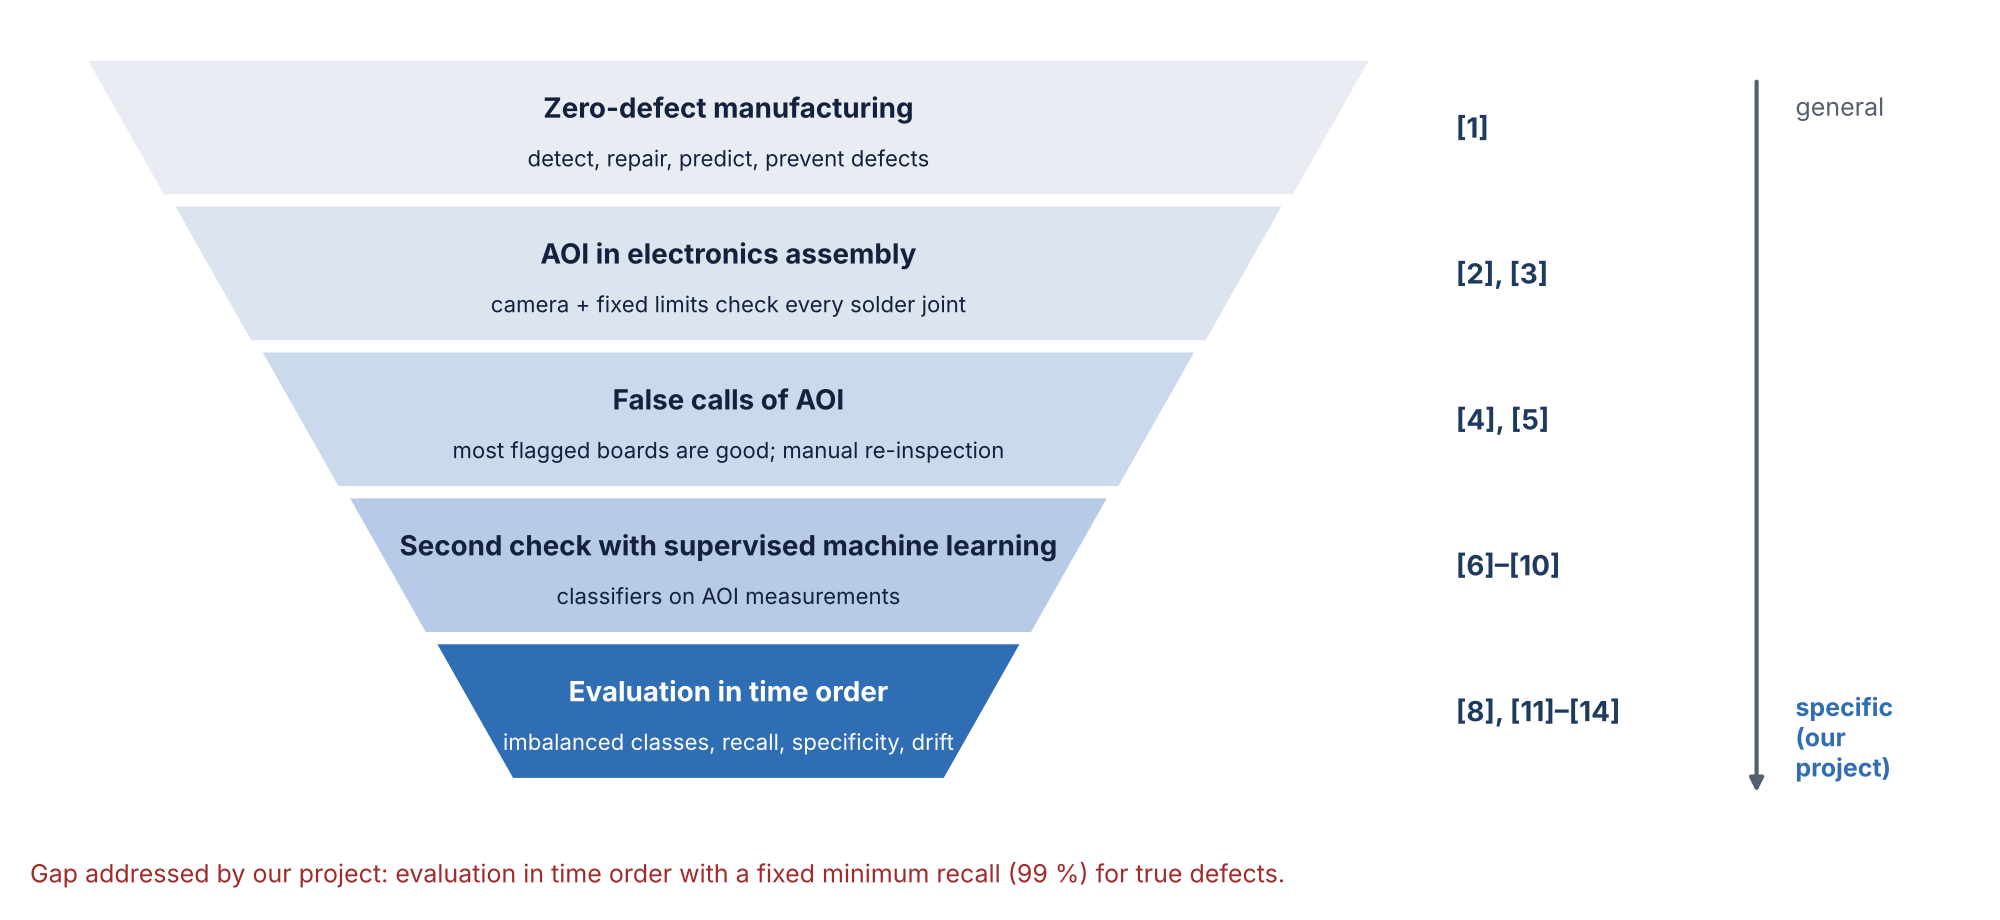
\includegraphics[width=0.95\textwidth]{literature_map.png}
  \caption{Reviewed literature from general to specific (numbers refer to the reference list).}
  \label{fig:map}
\end{figure}

% --- 2.2.1
\subsubsection{From zero-defect manufacturing to AOI in electronics assembly}

\source{Zero defect manufacturing: state-of-the-art review}{F.~Psarommatis et al. (2020), Int.\ J.\ Production Research}{\cite{psarommatis2020}}
The authors review 280 articles on zero-defect manufacturing published between 1987 and 2018. They group the approaches into four strategies: detection, repair, prediction and prevention of defects. They also note that most research looks at one strategy alone and that the role of people in quality control is rarely considered.
\relevance{AOI and the manual inspection station belong to the \textit{detection} strategy. Our second check makes detection cheaper (fewer manual checks of good boards) without letting more defects pass.}

\source{A review and analysis of automatic optical inspection and quality monitoring methods in electronics industry}{A.~A.~R.~M.~Abu Ebayyeh and A.~Mousavi (2020), IEEE Access}{\cite{ebayyeh2020}}
This review describes AOI systems in electronics production, including printed circuit boards: the hardware (cameras and lighting) and the software steps (pre-processing, feature extraction, classification). AOI replaces human visual inspection, which is slow and suffers from fatigue. The review also shows a trend from fixed rules towards machine learning in the classification step.
\relevance{It explains where our input comes from: AOI measures each solder joint and classifies it with fixed limits; our classifier works on these measurements after the AOI.}

\source{Short review on machine learning optimization methods in surface mounted electronics assembly technologies}{P.~Martinek et al. (2023), ISSE}{\cite{martinek2023}}
This short review collects machine learning applications along the SMT line, for example the tuning of stencil printing and component placement parameters and the control of production. It states that much research has used machine learning, such as artificial neural networks, to improve AOI.
\relevance{It places our project in a known field of research: machine learning applied to the inspection step of the SMT line.}

\source{Siemens and NVIDIA advance AI-powered PCB inspection from digital twin to factory}{Siemens (Oct.~2026), press release}{\cite{siemens2026}}
Siemens and NVIDIA prepare AOI programs on the computer, with a virtual ``golden board'' and synthetic images, before the first real board is produced; the solution is shown in the Siemens electronics factory in Erlangen. When the AOI flags a possible defect, a second inspection step decides whether it is a real defect or a false call. The stated targets are up to 85\,\% less manual engineering effort for AOI programs, 40\,\% fewer false calls and more than 5\,\% higher first-pass yield.
\relevance{It shows that the false-call problem is a current industrial problem. Our project makes the same decision (true defect or false call) with public data. The 40\,\% is a target, not a published result.}

% --- 2.2.2
\subsubsection{False calls of AOI: the Siemens data and earlier studies}

\source{Data of automated optical inspection of surface-mounted technology electronic production}{K.~Pfab et al. (2024), Data in Brief}{\cite{pfab2024}}
The authors publish 132 days of AOI data from one real SMT line of Siemens AG in Germany. Every row is a solder joint that the AOI flagged, with about 70 AOI measurements, and the label from the manual inspection station: true defect or false call. The authors warn that the labels were set by people, so the share of wrong labels is unknown, and that the data may contain changes over time (drift) of unknown type. In our own count the data contain 440,274 flagged solder joints on 39,742 boards; only 0.3--2.7\,\% of the joints are true defects, depending on the inspection type, and 97.8\,\% of the flagged boards are false calls.
\relevance{This is our data set. The possible drift and label errors are the reasons why we test in time order and why 99\,\% recall may be hard to keep.}

\source{A machine learning based approach to detect false calls in SMT manufacturing}{N.~Thielen et al. (2020), ISSE}{\cite{thielen2020}}
The authors test whether a machine learning step after the AOI can recognise false calls from the numerical AOI measurements. They compare k-nearest neighbours, an artificial neural network and random forests, and vary the data set size and the decision threshold. The aim is to recognise as many false calls as possible without more missed defects (slip). k-nearest neighbours works best on small data sets but becomes too slow on large ones, where neural networks and random forests perform better.
\relevance{It is the same task on the same kind of data, and it also fixes the missed defects first and counts the saved checks second, as our 99\,\% recall rule does. Its data are small and not public.}

\source{Enhancing false call detection in automated optical inspection using XGBoost classifier and XAI algorithms}{J.~Albayari et al. (FAIM 2025, publ.\ 2026), Springer LNME}{\cite{albayari2026}}
The authors use AOI data from Siemens AG and train classifiers as a second check after the AOI: XGBoost (gradient boosting), random forest, a deep neural network and k-nearest neighbours. They remove irrelevant and highly correlated features and test several train--test splits. XGBoost gives the best balance of recall and precision, and the methods LIME and SHAP show which AOI measurements drive the predictions.
\relevance{It applies the same classifier types to Siemens AOI data. It does not report a day-by-day evaluation in time order, which is the step our project adds.}

\source{Towards improved research methodologies for industrial AI: a case study of false call reduction}{K.~Pfab and M.~Rothering (2025), arXiv preprint}{\cite{pfab2025}}
Using the Siemens data from \cite{pfab2024}, the authors list seven weaknesses of earlier false-call studies, among them unpublished data and code, standard metrics instead of business goals, no clear success criteria, thresholds tuned on the test data and no analysis of changes over time. They set a goal of at least 40\,\% fewer manual checks with at most 1\,\% missed defects and train k-nearest neighbours, random forests, XGBoost and an AutoML model. Two random-forest models meet the goal on a random test set, but on five later time slices they miss 5--15\,\% of the defects, so they would fail in production.
\relevance{This is the most important source for our design: same data, a fixed recall goal, a threshold set on separate data, and evaluation in time order. It also warns that our goal of 99\,\% recall may be hard to keep on later days.}

% --- 2.2.3
\subsubsection{Supervised classifiers for the second check}

\source{Scikit-learn: machine learning in Python}{F.~Pedregosa et al. (2011), J.\ Machine Learning Research}{\cite{pedregosa2011}}
The paper introduces scikit-learn, an open-source Python library with a consistent interface for many standard machine learning methods, including logistic regression, random forests and multi-layer perceptrons (neural networks), together with tools for pre-processing and evaluation.
\relevance{All three classifiers of our project, and the data preparation, come from scikit-learn, so every step uses standard, documented code.}

\source{Random forests}{L.~Breiman (2001), Machine Learning}{\cite{breiman2001}}
A random forest is a set of decision trees. Each tree is trained on a random sample of the data and uses a random subset of the input features at each split; the trees then vote. The method is accurate on tabular data, needs little tuning and gives a measure of feature importance.
\relevance{The random forest performed well in \cite{thielen2020} and was the best model in \cite{pfab2025} and is one of our three classifiers; its feature importance is used later in our project.}

% --- 2.2.4
\subsubsection{Evaluation with imbalanced classes and changing data}

\source{Learning from imbalanced data}{H.~He and E.~A.~Garcia (2009), IEEE Trans.\ Knowledge and Data Engineering}{\cite{he2009}}
This review explains why accuracy is misleading when one class is rare, and presents methods such as class weighting and resampling. It recommends metrics that look at each class separately, such as recall (sensitivity), specificity, precision and ROC or precision--recall curves.
\relevance{True defects are about 1\,\% of the flagged joints. We therefore use class weighting and report recall (true defects caught) and specificity (false calls correctly classified) instead of accuracy.}

\source{An introduction to ROC analysis}{T.~Fawcett (2006), Pattern Recognition Letters}{\cite{fawcett2006}}
The paper explains how a classifier that gives a score is turned into a decision by a threshold, and how the threshold moves the result along the ROC curve: a lower threshold catches more positives (higher recall) but also gives more false alarms (lower specificity).
\relevance{Our classifier gives each board a score; we choose the threshold so that recall is 99\,\% and then measure the specificity reached at this point.}

\source{A survey on concept drift adaptation}{J.~Gama et al. (2014), ACM Computing Surveys}{\cite{gama2014}}
This survey describes learning when the data change over time (concept drift). It covers drift detection, how much past data to keep (memory) and how to update models, and it describes evaluation in time order, where the model is always tested on data that come after its training data.
\relevance{It is the basis of our day-by-day simulation (walk-forward evaluation): each production day is classified by a model trained only on earlier days.}

\source{Learning under concept drift: a review}{J.~Lu et al. (2019), IEEE Trans.\ Knowledge and Data Engineering}{\cite{lu2019}}
The review defines types of drift (sudden, gradual, incremental and recurring) and groups adaptation methods, from simple retraining on a recent window of data to ensembles and online updates.
\relevance{It supports our comparison of ``train once'' and ``retrain every week'' and our planned experiment with different training windows.}

\subsection{Summary of the reviewed works}
Table~\ref{tab:summary} compares the four studies that work directly on AOI false calls. Table~\ref{tab:methods} lists the methods of our project and the sources they come from.

\begin{table}[h]
\centering\small
\caption{Studies on AOI false calls compared with our project.}
\label{tab:summary}
\begin{tabularx}{\textwidth}{@{}p{2.3cm}LLLL@{}}
\toprule
 & Data & Classifiers & Test split & Success criterion \\
\midrule
Thielen et al.\ \cite{thielen2020} & small, not public & kNN, neural network, random forest & not stated & no extra slip \\
Albayari et al.\ \cite{albayari2026} & Siemens AG & XGBoost, random forest, DNN, kNN & several train--test splits & balance of recall and precision \\
Pfab \& Rothering \cite{pfab2025} & Siemens, public \cite{pfab2024} & kNN, random forest, XGBoost, AutoML & random test set + 5 later time slices & $\geq$40\,\% fewer checks, $\leq$1\,\% slip \\
\textbf{Our project} & Siemens, public \cite{pfab2024} & logistic regression, random forest, neural network & \textbf{day by day in time order} & \textbf{recall $\geq$99\,\%, specificity $\geq$20\,\%} \\
\bottomrule
\end{tabularx}
\end{table}

\begin{table}[h]
\centering\small
\caption{Methods of our project and the sources they are based on.}
\label{tab:methods}
\begin{tabularx}{\textwidth}{@{}p{4.6cm}Lp{2.3cm}@{}}
\toprule
Method in our project & Reason & Sources \\
\midrule
Binary classification: true defect or false call & the manual inspection label has exactly two classes & \cite{pfab2024,thielen2020} \\
Logistic regression, random forest, neural network (scikit-learn) & simple baseline plus the two model types that worked best in earlier studies & \cite{pedregosa2011,breiman2001,thielen2020,albayari2026} \\
Class weighting & true defects are rare & \cite{he2009} \\
Recall and specificity as KPIs & accuracy is misleading for rare classes & \cite{he2009,fawcett2006} \\
Threshold for 99\,\% recall, set on separate days & a missed defect is costly; no tuning on test data & \cite{fawcett2006,pfab2025} \\
Day-by-day evaluation in time order & production data change over time & \cite{gama2014,pfab2025} \\
Train once vs.\ retrain every week & adaptation to drift & \cite{lu2019,gama2014} \\
\bottomrule
\end{tabularx}
\end{table}

% ---------------- Conclusion ----------------
\section{Conclusion}
The literature leads from a general goal to a specific question. Zero-defect manufacturing needs reliable defect detection \cite{psarommatis2020}; in electronics assembly this is done by AOI \cite{ebayyeh2020,martinek2023}, which raises many false calls that operators must check by hand \cite{pfab2024}, a problem that industry is still working on today \cite{siemens2026}.

Earlier studies show that supervised machine learning can recognise false calls from AOI measurements, with random forests, neural networks and gradient boosting as the strongest models \cite{thielen2020,albayari2026}. The literature also shows three weaknesses: the data are often small or not public; models are not tested in time order, so past and future data can be mixed; and success is measured with standard metrics instead of a fixed goal for missed defects \cite{pfab2025}. When the same models are tested on later production days, the share of missed defects rises from about 1\,\% to 5--15\,\% \cite{pfab2025}, which agrees with the drift literature \cite{gama2014,lu2019}.

\textbf{Research gap addressed by our project:} a second check of AOI results that is evaluated as it would run on the line, day by day in time order on the public Siemens data, with a fixed minimum recall of 99\,\% for true defects and specificity as the measure of saved manual inspections \cite{he2009,fawcett2006}. Our first baseline already confirms the gap: at 99\,\% recall, the same three classifiers reach a specificity of 14--18\,\% with a random split but only 1.8--6.4\,\% in time order (results in our GitHub repository). The next steps of the project, such as thresholds per inspection type and different retraining windows, build directly on the sources reviewed here.

% ---------------- References ----------------
\begin{thebibliography}{99}
\addcontentsline{toc}{section}{References}
\small

\bibitem{psarommatis2020}
F.~Psarommatis, G.~May, P.-A.~Dreyfus, and D.~Kiritsis, ``Zero defect manufacturing: state-of-the-art review, shortcomings and future directions in research,'' \textit{Int.\ J.\ Production Research}, vol.~58, no.~1, pp.~1--17, 2020, doi:~10.1080/00207543.2019.1605228.

\bibitem{ebayyeh2020}
A.~A.~R.~M.~Abu Ebayyeh and A.~Mousavi, ``A review and analysis of automatic optical inspection and quality monitoring methods in electronics industry,'' \textit{IEEE Access}, vol.~8, pp.~183192--183271, 2020, doi:~10.1109/ACCESS.2020.3029127.

\bibitem{martinek2023}
P.~Martinek, I.~M.~Putrama, O.~Krammer, and A.~G\'eczy, ``Short review on machine learning optimization methods in surface mounted electronics assembly technologies,'' in \textit{Proc.\ 46th Int.\ Spring Seminar on Electronics Technology (ISSE)}, 2023, pp.~1--6, doi:~10.1109/ISSE57496.2023.10168524.

\bibitem{siemens2026}
Siemens, ``Siemens and NVIDIA advance AI-powered PCB inspection from Digital Twin to factory,'' press release, Plano, TX, USA, Oct.~21, 2026. [Online]. Available: \url{https://news.siemens.com/en-us/siemens-nvidia-pcba-digital-twin-factory/}

\bibitem{pfab2024}
K.~Pfab, R.~Eichler, A.~Mallandur, and M.~Rothering, ``Data of automated optical inspection of surface-mounted technology electronic production,'' \textit{Data in Brief}, vol.~53, Art.~no.~110110, Apr.~2024, doi:~10.1016/j.dib.2024.110110. Data: Mendeley Data, v2, doi:~10.17632/99jzmh9658.2.

\bibitem{thielen2020}
N.~Thielen, D.~Werner, K.~Schmidt, R.~Seidel, A.~Reinhardt, and J.~Franke, ``A machine learning based approach to detect false calls in SMT manufacturing,'' in \textit{Proc.\ 43rd Int.\ Spring Seminar on Electronics Technology (ISSE)}, Demanovska Valley, Slovakia, 2020, pp.~1--6, doi:~10.1109/ISSE49702.2020.9121044.

\bibitem{albayari2026}
J.~Albayari, P.~Patra, D.~Patel, and D.~Santos, ``Enhancing false call detection in automated optical inspection using XGBoost classifier and XAI algorithms,'' in \textit{Flexible Automation and Intelligent Manufacturing (FAIM 2025)}, Lecture Notes in Mechanical Engineering. Cham, Switzerland: Springer, 2026, pp.~509--530, doi:~10.1007/978-3-032-05610-8\_51.

\bibitem{pfab2025}
K.~Pfab and M.~Rothering, ``Towards improved research methodologies for industrial AI: a case study of false call reduction,'' arXiv:2506.14521 [cs.LG], Jun.~2025. [Online]. Available: \url{https://arxiv.org/abs/2506.14521}

\bibitem{pedregosa2011}
F.~Pedregosa \textit{et al.}, ``Scikit-learn: machine learning in Python,'' \textit{J.\ Machine Learning Research}, vol.~12, pp.~2825--2830, 2011.

\bibitem{breiman2001}
L.~Breiman, ``Random forests,'' \textit{Machine Learning}, vol.~45, no.~1, pp.~5--32, 2001, doi:~10.1023/A:1010933404324.

\bibitem{he2009}
H.~He and E.~A.~Garcia, ``Learning from imbalanced data,'' \textit{IEEE Trans.\ Knowledge and Data Engineering}, vol.~21, no.~9, pp.~1263--1284, Sep.~2009, doi:~10.1109/TKDE.2008.239.

\bibitem{fawcett2006}
T.~Fawcett, ``An introduction to ROC analysis,'' \textit{Pattern Recognition Letters}, vol.~27, no.~8, pp.~861--874, Jun.~2006, doi:~10.1016/j.patrec.2005.10.010.

\bibitem{gama2014}
J.~Gama, I.~\v{Z}liobait\.{e}, A.~Bifet, M.~Pechenizkiy, and A.~Bouchachia, ``A survey on concept drift adaptation,'' \textit{ACM Computing Surveys}, vol.~46, no.~4, Art.~no.~44, pp.~1--37, 2014, doi:~10.1145/2523813.

\bibitem{lu2019}
J.~Lu, A.~Liu, F.~Dong, F.~Gu, J.~Gama, and G.~Zhang, ``Learning under concept drift: a review,'' \textit{IEEE Trans.\ Knowledge and Data Engineering}, vol.~31, no.~12, pp.~2346--2363, Dec.~2019, doi:~10.1109/TKDE.2018.2876857.

\end{thebibliography}

\end{document}
